\documentclass[openany]{article}

%Typesetting and language
\usepackage[american]{babel}
\usepackage[T1]{fontenc}
\usepackage{charter}
\usepackage{enumitem}
\usepackage{hyperref}

%Symbols
\usepackage{amssymb, amsmath, amsthm, bm}
\usepackage{mathrsfs}
\usepackage{mathtools}
\usepackage{marvosym}
\usepackage{MnSymbol}

%Colors & graphics
\usepackage[dvipsnames]{xcolor}
\usepackage{pgfplots}
\usepackage[numbered,framed]{matlab-prettifier}
\usepackage{pgfplots}
\usepackage{listings}
\usepackage{tikz}
\usetikzlibrary{arrows.meta}
\usepackage[object=vectorian]{pgfornament}
\usepackage{wrapfig}
\usepackage{varwidth}
\usepackage[framemethod=TikZ]{mdframed}
\usepackage{caption}
\usepackage{float}
\usepackage{geometry}
\usepackage{ulem}
\usepackage[most]{tcolorbox}
\usepackage{array}

\setlength{\parindent}{0pt}

\makeatletter
\g@addto@macro\bfseries{\boldmath}
\makeatother


\renewcommand{\Re}{\mathfrak{Re}}
\renewcommand{\Im}{\mathfrak{Im}}

\geometry{left=2cm,right=2cm,bottom=2cm,top=2cm}

\usepackage{fancyhdr}
\pagestyle{fancy}
\fancyhf{}
\renewcommand{\sectionmark}[1]{\markright{\arabic{section} - #1}}
\cfoot{\thepage}
\lhead{CS270}
\chead{HW6}
\rhead{Adam Yang}
\renewcommand{\headrulewidth}{1pt}


\DeclareMathOperator{\sgn}{sgn}
\DeclareMathOperator{\im}{im}
\DeclareMathOperator{\var}{var}
\DeclareMathOperator{\Orb}{Orb}
\DeclareMathOperator{\Fix}{Fix}
\DeclareMathOperator{\Stab}{Stab}
\DeclareMathOperator{\cov}{cov}
\DeclareMathOperator*{\esssup}{ess\,sup}
\DeclareMathOperator{\corr}{corr}
\DeclareMathOperator{\lik}{lik}
\DeclareMathOperator*{\argmin}{argmin}
\DeclareMathOperator*{\argmax}{argmax}

\newcommand{\niceline}[2]{%
		\nointerlineskip \vspace{.5\baselineskip}\hspace{\fill}
		{\color{#1}
				\resizebox{0.5\linewidth}{2ex}
				{{%
								{\begin{tikzpicture}
										\node  (C) at (0,0) {};
										\node (D) at (9,0) {};
										\path (C) to [ornament=#2] (D);
										\end{tikzpicture}}}}}%
		\hspace{\fill}
		\par\nointerlineskip \vspace{.5\baselineskip}
}

\definecolor{darkViolet}{HTML}{9400D3}
\newcommand{\sweetline}{%
		\noindent
		\begin{center}
				{\color{darkViolet}
						\resizebox{0.5\linewidth}{1ex}
						{{%
										{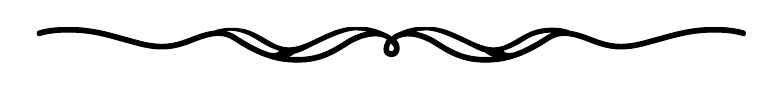
\begin{tikzpicture}
												\node  (C) at (0,0) {};
												\node (D) at (9,0) {};
												\path (C) to [ornament=85] (D);
												\end{tikzpicture}}}}}%
		\end{center}
}

\definecolor{remarkPurple}{HTML}{8346FF}
\definecolor{defBlue}{HTML}{0673FF}
\definecolor{exPurple}{HTML}{FF8710}

%THEOREM
\newtcbtheorem[auto counter,number within=section]{theorem}{Theorem}%
{enhanced,colback=white, breakable,frame empty,interior empty,colframe=cyan!50!white, top=8mm,
				coltitle=black,fonttitle=\bfseries,colbacktitle=cyan!15!white,
				borderline={0.5mm}{0mm}{cyan!15!white},
				borderline={0.5mm}{0mm}{cyan!50!white,dashed},
				attach boxed title to top left={yshift=-4mm},
				boxed title style={sharp corners=east,boxrule=1pt},varwidth boxed title}{thm}

%PROPOSITION
\newtcbtheorem[use counter from=theorem]{proposition}{Proposition}%
{enhanced,colback=white,breakable,frame empty,interior empty,colframe=defBlue!75!white, top=8mm,
				coltitle=black,fonttitle=\bfseries,colbacktitle=defBlue!20!white,
				borderline={0.5mm}{0mm}{defBlue!20!white},
				borderline={0.5mm}{0mm}{defBlue!50!white,dashed},
				attach boxed title to top left={yshift=-4mm},
				boxed title style={sharp corners=east,boxrule=1pt},varwidth boxed title}{prop}

%DEFINITION
\newtcbtheorem[use counter from=theorem]{definition}{Definition}%
{enhanced,colback=white,breakable,frame empty,interior empty,colframe=defBlue!75!white, top=8mm,
				coltitle=black,fonttitle=\bfseries,colbacktitle=defBlue!20!white,
				borderline={0.5mm}{0mm}{defBlue!20!white},
				borderline={0.5mm}{0mm}{defBlue!50!white,dashed},
				attach boxed title to top left={yshift=-4mm},
				boxed title style={sharp corners=east,boxrule=1pt},varwidth boxed title}{def}

%COROLLARY
\newtcbtheorem[use counter from=theorem]{corollary}{Corollary}%
{enhanced,colback=white,breakable,frame empty,interior empty,colframe=defBlue!75!white, top=8mm,
				coltitle=black,fonttitle=\bfseries,colbacktitle=defBlue!20!white,
				borderline={0.5mm}{0mm}{defBlue!20!white},
				borderline={0.5mm}{0mm}{defBlue!50!white,dashed},
				attach boxed title to top left={yshift=-4mm},
				boxed title style={sharp corners=east,boxrule=1pt},varwidth boxed title}{cor}

%REMARK
\newtcbtheorem[no counter]{remark}{Remark}%
{detach title, colback=white,enhanced ,breakable,frame empty, interior empty, fonttitle=\bfseries, coltitle=Violet, before upper={\tcbtitle.\quad},
				borderline west={0.5mm}{0mm}{remarkPurple!40!white},
				borderline west={0.5mm}{0mm}{remarkPurple!60!white,dashed}}{remark}

%LEMMA
\makeatletter
\newtcbtheorem[number within = tcb@cnt@theorem]{lemma}{Lemma}%
{enhanced,breakable,colback=white,frame empty,interior empty,colframe=orange!75!white, top=8mm,
				coltitle=black,fonttitle=\bfseries,colbacktitle=orange!20!white,
				borderline={0.5mm}{0mm}{orange!20!white},
				borderline={0.5mm}{0mm}{orange!50!white,dashed},
				attach boxed title to top left={yshift=-4mm},
				boxed title style={sharp corners=east,boxrule=1pt},varwidth boxed title}{lemma}
\makeatother


%PROOF
%%{enhanced,breakable,frame empty,interior empty,colframe=remarkPurple!75!white, top=8mm,
%	coltitle=black,fonttitle=\bfseries,colbacktitle=remarkPurple!20!white,
%	borderline={0.5mm}{0mm}{remarkPurple!20!white},
%	borderline={0.5mm}{0mm}{remarkPurple!50!white,dashed},
%	attach boxed title to top left={yshift=-4mm},
%	boxed title style={sharp corners=east,boxrule=1pt},varwidth boxed title}{prf}


\tcolorboxenvironment{proof}{% amsthm' 
				blanker,breakable,left=5mm,
				before skip=10pt,after skip=10pt,
				borderline west={0.5mm}{0pt}{cyan!40},
				borderline west={0.5mm}{0pt}{remarkPurple!10, dashed}}

%PROBLEM
\newtcbtheorem[auto counter]{problem}{Problem}%
{enhanced,breakable,colback=white,frame empty,interior empty,colframe=cyan!50!white, top=8mm,
				coltitle=black,fonttitle=\bfseries,colbacktitle=cyan!20!white,
				borderline={0.5mm}{0mm}{cyan!20!white},
				borderline={0.5mm}{0mm}{cyan!50!white,dashed},
				attach boxed title to top left={yshift=-4mm},
				boxed title style={sharp corners=east,boxrule=1pt},varwidth boxed title}{prob}

%EXAMPLE
%\newtcbtheorem[use counter from=problem]{example}{Example}%
%{enhanced,breakable,colback=white,frame empty,interior empty,colframe=remarkPurple!50!white, top=8mm,
%		coltitle=black,fonttitle=\bfseries,colbacktitle=remarkPurple!30!white,
%		borderline={0.5mm}{0mm}{remarkPurple!30!white},
%		borderline={0.5mm}{0mm}{remarkPurple!30!white,dashed},
%		attach boxed title to top left={yshift=-4mm},
%		boxed title style={sharp corners=east,boxrule=1pt},varwidth boxed title}{ex}


\newtcbtheorem[use counter from=theorem]{example}{Example}%
{detach title, colback=white,enhanced ,breakable,frame empty, interior empty, fonttitle=\bfseries, coltitle=black, before upper={\tcbtitle.\quad},
		borderline west={0.5mm}{0mm}{remarkPurple!30!white},
		borderline ={0.5mm}{0mm}{remarkPurple!30!white}}{example}

%SOLUTION
\newtcbtheorem[no counter]{solution}{Solution}%
{enhanced,breakable,colback=white,frame empty,interior empty,colframe=green!75!white, top=8mm,
				coltitle=black,fonttitle=\bfseries,colbacktitle=green!20!white,
				borderline={0.5mm}{0mm}{green!20!white},
				borderline={0.5mm}{0mm}{green!50!white,dashed},
				attach boxed title to top left={yshift=-4mm},
				boxed title style={sharp corners=east,boxrule=1pt},varwidth boxed title}{sol}
\definecolor{realPurple}{HTML}{AA05F9}
\definecolor{gray}{rgb}{0.5,0.5,0.5}
\definecolor{dkgreen}{rgb}{0,0.6,0}
\definecolor{mauve}{rgb}{0.58,0,0.82}

\lstset{frame=tb,
				style=Matlab-editor,
				language=C,
				aboveskip=3mm,
				belowskip=3mm,
				xleftmargin=3mm,
				showstringspaces=false,
				columns=flexible,
				frame=none,
				basicstyle={\small\ttfamily},
				numberstyle=\tiny\color{gray},
				keywordstyle=\color{blue},
				commentstyle=\color{dkgreen},
				stringstyle=\color{mauve},
				breaklines=true,
				breakatwhitespace=true,
				mlshowsectionrules = true,
				tabsize=3,
				backgroundcolor=\color{cyan!5}
}

\newcommand\mmybox[2][fill=cyan!20]{%
    \tikz[baseline]\node[%
        inner ysep=0pt, 
        inner xsep=2pt, 
        anchor=text, 
        rectangle, 
        rounded corners=1mm,
        #1] {\strut#2};%
}


\def\changemargin#1#2{\list{}{\rightmargin#2\leftmargin#1}\item[]}
\let\endchangemargin=\endlist

\linespread{1.4}



% MAIN DOC
\begin{document}

\title{HW 6}
\author{Adam Yang}
% \date{\today}
\maketitle




\section*{Problem1}

In the following answer, denote $n$ as total days to detect, $k$ as total target days of drought, $p_i\in [0,1]$ as the probability of rain in $i$-th day, $i\in [0,n]$ $\Rightarrow (1-p_i)$ is the probability of drought on $i$-th day. All $p_i$ are independent. We will focus on number of drought days in the following discussion.

\subsection*{Algorithm}
\begin{proof}[Algorithm]{}
		\renewcommand{\qedsymbol}{}
		An Algorithm to compute the probability that more than k days will be drought days in 2023
		\begin{lstlisting}[basicstyle=\fontsize{8}{9}\selectfont\ttfamily]
/**
* p[] is the input probability list, p[i] stores probability p_i of raining in i-th day, index from 0 to n, p[0] = 0
* n is the observing days
* k is the targeting days
* in the following code, dp[i][j] stores the probability that i days have exactly j days drought
**/
float findProb(float[] p, int n, int k){
    if(k>n) return 0; // edge case
	 float[][] dp = new dp[n+1][n+1]; // +1 for extra 0 bases
    set (n+1)*(k+1) all entry in dp[][] to 0;
    dp[0][0] = 1;
    dp[1][0] = p[1]; // 1 day AND 0 day drought = p_1
    dp[1][1] = 1-p[1]; // 1 day AND 1 day drought = 1-p_1
    // initialization
    for(int i = 2; i <= n; ++i){
      dp[i][0] = dp[i-1][0] * p[i];
      dp[i][i] = dp[i-1][i-1] * (1-p[i]);
    }
    // start finding
    for(int i = 1; i <= n; ++i){
      for(int j = 1; j < i; ++j){ // never reach dp[i][i], which has been initialized
          dp[i][j] = dp[i-1][j]*p[i] + dp[i-1][j-1]*(1-p[i]);
      }
    }
    float res;
    for(int i = k+1; i <= n; i++) res += dp[n][i];
    return res;
}

        
		\end{lstlisting} 
\end{proof}

\subsection*{Proof}
\begin{proof}[Correctness]{}
The goal is to find the probability of more than $k$ days are drought in n days.

\textbf{Definition:} Let $X$ be the number of drought days, $P_i(X=j)$ be the probability of there are $j$ days drought in $i$ day, $R$ be the event of raining, $D$ be the event of drought. Notice that $R_i=D_i^c$.

Since the raining and drought in each day is independent \[P_n(k<X\leq n) = P_n(X=k+1, X=k+2, ..., X= n)\] \[= P_n(X=k+1) + ... + P_n(X=n) = \sum_{j=k+1}^{n}P_n(X=j), k \leq n\]

Notice that it is impossible to have k days drought in n days if $k>n$, therefore $P_n(X\leq n < k) = 0$ Since this is vacuously true to say the probability is zero, the following discussion will only focus on $k\leq n$ scenario.

\textbf{Sub-problem:} Define the sub-problem $(i,j)$ to be finding the probability that there are exactly $j$ drought days in $i$ days, $i\in[0,n]$.
    
\textbf{Recurrence Relation:} With the probability of $j$ days drought in $i$ days,  $0\leq j<i\leq n$ as $P_i(X=j)$.

1. If $i$-th day is raining, then there have been $j$ days drought already in previous $i-1$ days.

2. If $i$-th day is drought, then there have been $j-1$ days drought already in previous $i-1$ days.

Thus, the probability that there are exactly $j$ drought days in $i$-th day is \[P_i(X=j) = P_{i-1}(X=j|R_i) + P_{i-1}(X=j-1|D_i)\]
\[=p_i\cdot P_{i-1}(X=j) + (1-p_i)\cdot P_{i-1}(X=j-1)\]

Therefore, the probability that exactly $k$ days are drought in $n$ days has the recurrence relation:
\[P_n(X=k) = p_n\cdot P_{n-1}{X=k} + (1-p_n)\cdot P_{i-1}{X=k-1}, i\leq n\]
    
    
\textbf{Base Cases:}

1. There is zero drought day in zero day. $P_0(X=0)=1$

2. There is zero drought day in one day. $P_1(X=0)=p_1$

3. There is one drought day in one day. $P_1(X=1)=1-p_1$

4. There is zero drought day in $i$ day, $i\in[1,n]$, $P_i(X=0)=p_i\cdot P_{i-1}(X=0) = \prod_{k=1}^{i}p_k$ by independence

5. There is $i$ day drought in $i$ day, $i\in[2,n]$,
$P_i(X=i)=(1-p_i)\cdot P_{i-1}(X=i-1) = \prod_{k=1}^{i}(1-p_k)$ by independence
    
\textbf{Edge Case}:

1. There are $j$ drought days in $i$ days, $i<j$. $P_i(X=j) = 0$

\textbf{Correctness Proof:}

Correctness statement: $\sum_{j=k+1}^{n}$dp[$n$][$j$] = $P_n(k<X\leq n)$
  
We will prove along the way: dp[$i$][$j$] = $P_i(X=j)$ for all $ 0 \leq j < i \leq n$

\textbf{Proof by induction on $i+j$:}

\textbf{Inductive Hypothesis:} For all $0 \leq i'+j'<i+j,0 \leq j \leq i \leq n$, dp[$i'$][$j'$] = $P_{i'}(X=j')$

\textbf{Base Cases:}

1. dp[0][0] = 1 = $P_0(X=0)$

2. dp[1][0] = $p_1$ = $P_1(X=0)$

3. dp[1][1] = $1-p_1$ = $P_1(X=1)$

\textbf{Inductive Cases:}

1. $i$ days have $j$ drought days ($i>j$): \\ \texttt{dp[i][j]} = $p_i \cdot$ dp[i-1][j] + $(1-p_i) \cdot$ dp[i-1][j-1] \textbf{\textit{*by Assignment*}} \\= $p_i\cdot P_{i-1}(X=j) + (1-p_i)\cdot P_{i-1}(X=j-1)$ \textbf{\textit{*by Inductive Hypothesis, $i+j-1 < i+j, i+j-2 < i+j$*}}
\\= $P_i(X=j)$ \textbf{\textit{*by Recurrence Relation*}}

2. $i$ days have 0 drought days: \texttt{dp[i][0]} = $p_i \cdot$ dp[i-1][0] =  $p_i\cdot P_{i-1}(X=0)$ = $P_i(X=0)$ for $2\leq i \leq n$ (no drought day) \textbf{\textit{*by IH and Recurrence relation, $i-1 < i+j$*}}

3. $i$ days have $j=i$ drought days: \texttt{dp[i][i]} = $(1-p_i) \cdot$ dp[i-1][i-1]  = $p_i\cdot P_{i-1}(X=i-1)$ =   $P_i(X=i)$ for $2\leq i \leq n$  (all drought day) \textbf{\textit{*by IH and Recurrence relation, $i+j-2 < i+j$ *}}

4. $i$ days have $j$ drought days ($i>j$): \texttt{dp[i][j]} = 0 = $P_j(X=i)$

Thus, \texttt{dp[i][j]} = $P_i(X=j)$. for $0 \leq j \leq i \leq n, k \leq n$. Therefore, in the last for loop where we get the result to return,
\begin{center}
    \texttt{res =} $\sum_{i=k+1}^{n}$\texttt{dp[n][i]} = $\sum_{i=k+1}^{n}P_n(X=i) = P_n(k<X\leq n)$
\end{center}

This concludes the proof since the algorithm correctly return the probability that there are more than k drought days in n days.

\end{proof}
\begin{proof}[Termination]{}
    All-for-loop algorithm with finite repetition, vacuously true. It terminates.
\end{proof}

\subsection*{Running Time}
In this algorithm, all elementary calculation and assignment are considered $\mathcal{O}(1)$.

Line 8 - 13 (except 10) take $\mathcal{O}(1)$ declaration and assignment. Line 10 take $\mathcal{O}(n^2)$ initialization for a $n\times n$ matrix. Line 15-18 take $\mathcal{O}(n)$ for looping through $\{2,3,...,n\}$. Line 21 - 23 (inner for loop) take $\mathcal{O}(i)$. Line 20 - 24 take $\sum_{i=1}^{n}\mathcal{O}(i) = \mathcal{O}(n^2)$. Line 25 - 27 take $\mathcal{O}(n)$ for looping from $\{k+1,...,n\}$. Thus, the running time of algorithm is
\[T(n) = 3\mathcal{O}(n) + 2\mathcal{O}(n^2) = \mathcal{O}(n^2)\]


\section*{Problem2}

In the following answer, $G = (V,E)$ is the directed graph we will discuss and $x=x_1x_2\cdots x_T$ is the string to compute. Denote $|V|$ as $n$, $|E|$ as $m$, size of $x$ as $T$, starting node as $s$, $e(u,v)$ as an edge $u \rightarrow v$, $u,v\in V$. We store a 2D array \texttt{a[][]}. For convenience, all nodes have a unique corresponding index to refer back to a[$v$][$t$], $v\in V, t\in [0, T]$ (This can be easily achieved through assigning into an array in real implementation). Define a[$v$][$t$] stores the maximum likelihood of the sequence that starts with $s$ and end with $v$ for outputting $x_1\cdots x_t$. In this problem, we fix node $s$ as the starting point of the sequence $v_1$.

For each node $v\in V$, $v$ stores an array q[] for the likelihood of outputting a letter from 'a' to 'z'; and an p[] for the likelihood of picking an out-going edge to another node: $v$.q[$x$] is the probability of node $v$ output $x, x \in \{'a','b', \cdots, 'z'\}$; $v$.p[$u$] is the probability of node v goes to $u \neq v, u \in V$ through an out-going edge $e(v,u)$, if no such $e$ then $v$.p[$u$] = 0. 
\subsection*{Algorithm}
\begin{proof}[Algorithm]{}
		\renewcommand{\qedsymbol}{}
		An Algorithm to find the maximum likelihood of any vertex sequence for the given string
		\begin{lstlisting}[basicstyle=\fontsize{8}{9}\selectfont\ttfamily]
Define Graph G = (V,E) where V is the node set and E is the edge set;

// it is C++ like pseudo-code, max_element and push_back() are functions for vector<T> in STL
/**
* Graph G is the input G=(V,E)
* x is the input string to compute
* x indexed from 1 to T
**/

float findProb2(Graph G, String x){
    if(x.size() == 0) return 0; // zero possibility of no sequence
    n := size of V;
    m := size of E;
    T := size of x;
    initialize a 2D array a[n][T], set each place to 0;
    a[s][1] = s.q[x[1]];
    for(int t = 2; k <= T; k++){
        for(all node v in V){
            vector<float> temp; // help find max item
            
            // find max probability for v
            for(all node u S.T e(u,v) exists){ // u->v
                temp.push_back(a[u][t-1] * u.p[v] * s.q[x[t]]);
            }
            a[v][t] = max_element(temp.begin(), temp.end())
        }
    }
    float res = 0;
    for(all node v in V){
        if(a[v][T] > res) res = a[v][T];
    }
    return res;
}

        
		\end{lstlisting} 
\end{proof}

\subsection*{Proof}
\begin{proof}[Correctness]{} The goal is to find the maximum likelihood of any vertex sequence for the given string.

\textbf{Definition:} 
Define node $v_t$ as the ending vertex for the sequence that output $x_1\cdots x_t$. Since the system fix $s$ as the starting node $v_1$, we will only discus $t\geq 2$ below. For any node $v_t, t\geq 2$, $v_{t-1}$ is any node S.T. an edge $e(v_{t-1}, v_{t})$ exists; $v_{t+1}$ is any node S.T. an edge $e(v_t, v_{t+1})$ exists.

In the algorithm above, $\forall v,u\in V, v\neq u:$  we use $v$.p[$u$] to represent the probability that node $v$ goes to next node $u$. In the discussion below, we will use $p_{v_t,(v_t,v_{t+1})}$ to represent the likelihood of node $v_t$ going to next node $v_{t+1}$, $ t=\{1,2,...,T-1\}$. Similarly, we use $q_{v_t,x_t}$ replace $v.$q[x[t]] and represent the probability of node $v_t$ writing down $x_t$. (This is for easier mathematical calculation with mathematical languages)

By definition, the likelihood of a sequence $\langle v_1,v_2,...,v_T \rangle$ to output $x=x_1x_2\cdots x_T$
\[L(\langle v_1,v_2,...,v_T \rangle) = \prod_{t=1}^{T}q_{v_t,x_t} \cdot \prod_{t=1}^{T-1}p_{v_t,(v_t,v_{t+1})}  \]
    
\textbf{Sub-problem:} Define the sub-problem Opt($v_t, t$) as finding the maximum likelihood of the vertex sequence for the given string $x_1x_2\cdots x_t$ that end with $v_t$.

Define the sub-sub-problem $L(v_t,t)$ for finding Opt($v_t,t$) as finding the likelihood of the sequence where we fix $v_t\in V$ as the last vertex in the sequence for $x_1 \cdots x_t$.
    
\textbf{Recurrence Relation:} Focusing on the likelihood of any vertex sequence $L(v_t,t)$ for $x_1\cdots x_t$, we have

\[L(v_t,t)=L(\langle v_1,v_2,...,v_t \rangle)=
\prod_{t=1}^{t}q_{v_i,x_i} \cdot \prod_{t=1}^{t-1}p_{v_i,(v_i,v_{i+1})}\]
\[=q_{v_1,x_1}\cdot q_{v_2,x_2} \cdot ... \cdot q_{x_t, x_t} \cdot p_{v_1,(v_1, v_2)} \cdot ...\cdot p_{v_{t-1},(v_{t-1}, v_{t})}=\prod_{t=1}^{t-1}q_{v_i,x_i} \cdot \prod_{t=1}^{t-2}p_{v_i,(v_i,v_{i+1})} \cdot q_{v_t,x_t} \cdot p_{v_{t-1},(v_{t-1},v_t)}\]


\[= L(\langle v_1,v_2,...,v_{t-1} \rangle)\cdot q_{v_t,x_t} \cdot p_{v_{t-1},(v_{t-1},v_t)} \]
\[= L(v_{t-1}, t-1) \cdot q_{v_t,x_t} \cdot p_{v_{t-1},(v_{t-1},v_t)}  \]


From the equation above, we show the recurrence relation for sub-sub-problem $L(v_t,t)$ using mathematical relation. And we can conclude that probability of building a $t$-length vertex sequence to output $x_1\cdots x_t$ depends on the following three parts

\qquad 1. $L(v_{t-1},t-1)$, the likelihood of $t-1$ length sequence

\qquad 2. $q_{v_t, x_t}$, the likelihood of $v_t$ output $x_t$

\qquad 3. $p_{v_{t-1}, (v_{t-1}, v_t)}$, the likelihood of $v_{t-1}$ goes to $v_t$

Based on these three information, we can form our recurrence relation for finding maximum likelihood for any vertex sequence. For any $v_{t-1} \in V$, incur the probability of going from $v_{t-1}$ to $v_t$ and then output $x_t$ in $v_t$ as $p_{v_{t-1}, (v_{t-1},v_t)} \cdot q_{v_t,x_t}$; and for each $v_{t-1}\in V$, maximum likelihood of $L(v_{t-1},t-1) = Opt(v_{t-1},t-1)$ are found (optimally). Since there are many ways to form a vertex sequence that ends with $v_t$ for $x_1\cdots x_t$, we need to take care of all possible $Opt_{v_{t-1}\in V}(v_{t-1},t-1)$. From all possible ways to output $x_1\cdots x_t$ and ends with $v_t$, Opt($v_t,t$) choose the maximum probability from all possible $L(v_t, t)$. Therefore, the maximum likelihood of any vertex sequence of $x_1\cdots x_t$ by fixing vertex $v_t$ as the last vertex in the sequence have the following recurrence relation
\[Opt(v_t,t) = \mathop{\max}_{v_t\in V} \Bigg[ L(v_t,t) \Bigg]
= \mathop{\max}_{v_t\in V} \Bigg[ L(\langle v_1,...,v_{t} \rangle) \Bigg]  \]

\[= \mathop{\max}_{v_{t-1}\in V} \Bigg[ Opt(v_{t-1},t-1) \cdot q_{v_t,x_t} \cdot p_{v_{t-1},(v_{t-1},v_t)} \Bigg]\]

In the last step, now that we have all possible maximum vertex sequence to output $x_1\cdots x_t$ and end with n $Opt_{v\in V}(v,T)$, we are going to find the maximum likelihood path among them. Therefore, we will return the maximum likelihood p
\[p = \mathop{\max}_{v_{t}\in V} \Bigg[ Opt(v_{t},T)\Bigg]\]


\textbf{Base Case:}
$t = 1$: Since the system fix node $s$ as the starting vertex $v_1$ in the sequence, $s$ itself can only output $x_1$ and any other starting point has 0 likelihood. Thus, for the base case $x_1, t=1$
\[Opt(s,1) = L(s,1) = q_{s,x_1} , Opt_{v\in V, v\neq s}(v,1) = 0\]
    

\textbf{Correctness Proof:}
Base case, we assign \texttt{a[s][1]} as \texttt{s.q[x[1]]} = $q_{s,x_1} = Opt(s,1)$ and \texttt{a[v][1]} as 0 for $v\in V, v\neq s$. The recurrence relation is implemented from line 22 to 25 for finding the maximum likelihood of the vertex sequence ending at time $t$ on $v$. With induction, we can prove the correct assignment in the algorithm. Also, since this is algorithm will terminate since all for-loop are finite, a[v][t] indeed stores the $Opt(v,t)$. In order to find the maximum probability for outputting $x_1x_2\cdots x_T$, we only need to the maximum from all possible $Opt(v,t)$ and return. Therefore it is correct.
\end{proof}

\subsection*{Running Time}
Line 12-16 are $\mathcal{O}(nT)$ declaration and assignment. Line line 22-25, $\mathcal{O}(|V|) = \mathcal{O}(n)$ comparisons are required for finding the maximum one from all possible $L(v_{t-1},t-1)$. From line 18 to 26, the middle for-loop repeats $\mathcal{O}(n)$ times for looping through all the node and thus take $\mathcal{O}(n^2)$. From line 17 to 27, the outer for-loop repeats $\mathcal{O}(T)$ times and thus take $\mathcal{O}(Tn^2)$. From 29 to 32, it takes $\mathcal{O}(n)$ for checking all the node. Thus, the running time is:
\[T(n) = \mathcal{O}(1) + \mathcal{O}(n)+ \mathcal{O}(Tn^2) = \mathcal{O}(Tn^2)\]

From line 22-25, we can also say that we only need $\mathcal{O}(deg_{in}(v))$, and therefore from line 18 to 26 takes $\sum_{v\in V} \mathcal{O}(deg_{in}v) = \mathcal{O}(\frac{m}{2}) = \mathcal{O}(m)$. Therefore, from line 17 to 27 the run time is $\mathcal{O}(Tm)$. Therefore, the running time can also be
\[T(n) = \mathcal{O}(1) + \mathcal{O}(n)+ \mathcal{O}(Tm) = \mathcal{O}(Tm)\]

Notice that for $G=(V,E)$, $|E|=m=\mathcal{O}(n^2)$ (all node are connected to each other). Thus, $\mathcal{O}(Tm) = \mathcal{O}(Tn^2)$
\end{document}
